\graphicspath{{Figures/chapter2}}
\chapter{LITERATURE SURVEY}
This chapter discusses the various related works and previous studies conducted on Speed bump and Pothole Detection. A lot of studies can be seen in recent years for detecting speed bumps and potholes in the road surface automatically.

\noindent
\section{Sensor-based approaches}
 One of the major problems in developing
countries is road maintenance, most of the
accidents happen due to unmarked speed breakers in the
national highway which leads to a threat to drivers. An
Intelligent transportation system plays a vital role in the
advanced driver assistance system. The speed breaker
recognition is used for vehicle and human safety.
Earlier speed breaker detection method involves
sensors, accelerometers, and GPS. Getting into the first sensor-based study approach in this paper,  a novel
method for speed breaker detection and recognition is
developed to alert the driver before the vehicle hit the
speed breaker\cite{R11}. In BLOB analysis, image processing techniques are used to detect the speed breaker in the given image. The camera fixed in the vehicle is used to capture the image of the road and it is analysed in the real-time to detect the presence of speed breaker. This technique can be used for the painted speed breaker. Images captured using a single camera is analysed for finding the speed breakers. This method works fine for colored speed breakers whereas the performance is not up to the mark for uncolored speed breakers. Images taken from more than one camera can be used to improve accuracy. A classification algorithm can also be used for better detection of speed breakers.
\begin{figure}[H]
    \centering
    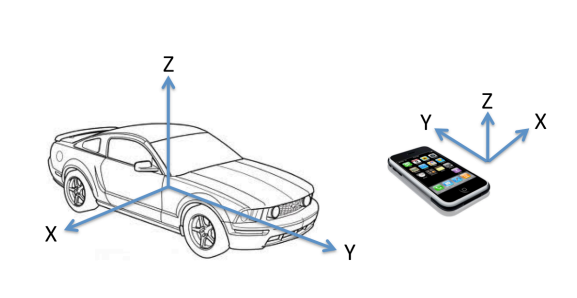
\includegraphics[scale=0.9]{Figures/chapter2/sensor.png}
    \caption{The three axes of a car and a smartphone}
    \label{fig:carsensor}
\end{figure}

\noindent
A system for detecting speed bumps and lanes on roads using HC-SR04 ultrasonic sensor and Wi-Fi sports camera respectively is presented in \cite{R18}. When the speed bump is close to the ultrasonic sensor, the sensor detects the speed bump and the ESP8266 Wi-Fi module transfers the location information to the cloud server through Google Geolocation API. A local database is used to detect the location coordinates of the speed bump.

\noindent
The next paper is the "Road Quality and Ghats
Complexity analysis using Android sensors"\cite{R5} which describes a mobile sensing system (android application) for road irregularity detection using Android OS based smart phone sensors. Selected data processing algorithms are discussed and their evaluation is presented with a true positive rate as high as 90 percent using real-world data. The optimal parameters for the algorithms are determined as well as recommendations for their application.Continuously keeping track on road and traffic conditions in a city is a problem widely studied. Many methods have available towards addressing this problem. But this methods proposed require dedicated hardware such as GPS devices and accelerometers in vehicles or cameras on roadside and near traffic signals. All such proposed are unaffordable to the common man regarding of monetary cost and human effort required. We extend a prior study to improve the algorithm based on using accelerometer, GPS and magnetometer sensor readings for traffic and road conditions detection. This paper explores features and relationships between acceleration data, collected by smartphones, and road roughness conditions. The assumption that a rough estimation of road surface conditions from smartphones would be helpful enough for road management and planning, provided that the approach is very low cost, easy to operate and can be implemented frequently.
\begin{figure}[h]
    \centering
    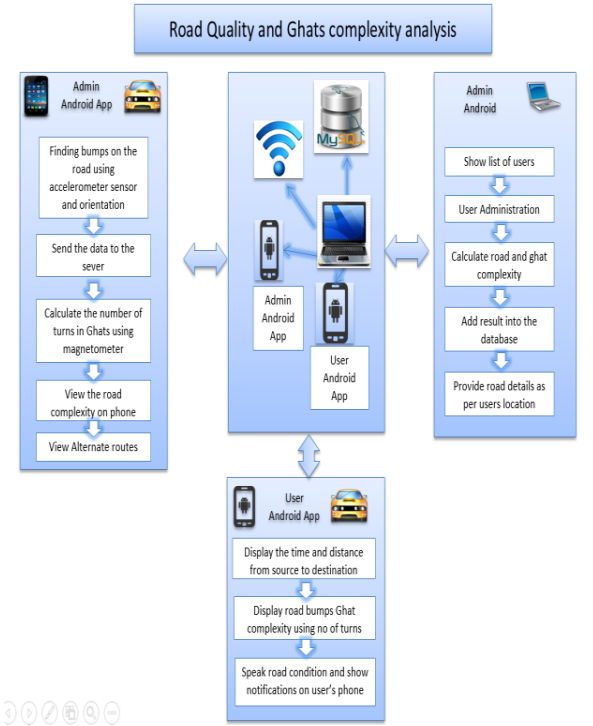
\includegraphics[scale=0.8]{Figures/chapter2/sensor1.png}
    \caption{continuous road condition monitoring system}
    \label{fig:sensor1}
\end{figure}

\noindent
Similarly, scheme of sensor’s signals on speed bump were detected using magnetometer, accelerometer, and GPS. Location and time label of the extracted data were then sent to the server that employed k-means clustering to process the sensor’s data \cite{R10}. In another study of sensors data, Manuel et al. engaged smartphone accelerometer to recognize several road anomalies. It consisted of sliding window method that pre-process the sensors data, then obtained the statistical features, and applied support vector machine (SVM) to classify those anomalies \cite{R6}. In another approach, Jose et al. deployed genetic algorithm (GA) and operated over accelerometer, gyro features, and GPS sensors data to spot speed bumps on the road \cite{R7}. To analyze road conditions; Luis et al. employed machine learning techniques and characterize the accelerometer data by feature pool as Bag of Words (BoW) \cite{R9}. Some of the studies involved smartphone based applications where inbuilt sensors were used to observe the fluctuation patterns of vehicle’s driving through variable road surfaces like speed humps, bumps, uneven roads, cracks, potholes, and smooth road. To counter imminent frontal impacts as an early warning system, smartphone based accelerometer sensors were processed.

\section{Vision-based approaches}
A novel supervision location-aware architecture is proposed for pothole detection \cite{R12}. The approach is based on an intuitive idea: identification of pavement potholes generally first tries to find regions that would more likely contain potholes, then amplifies these areas to a larger resolution and focuses on the discriminative parts to distinguish between areas that have potholes and areas that are pothole free. Such a situation requires tackling the object localization and classification problem as a two-stage process. The proposed approach is to localize the pothole regions under supervision of the center of each pothole. However, to obtain better classification results, it may be beneficial to fnd candidate object parts and focus on the discriminative regions instead of directly running the experiments on the whole image to be classified.More details of potholes are detected in the high-resolution than the low-resolution.
\begin{figure}[H]
    \centering
    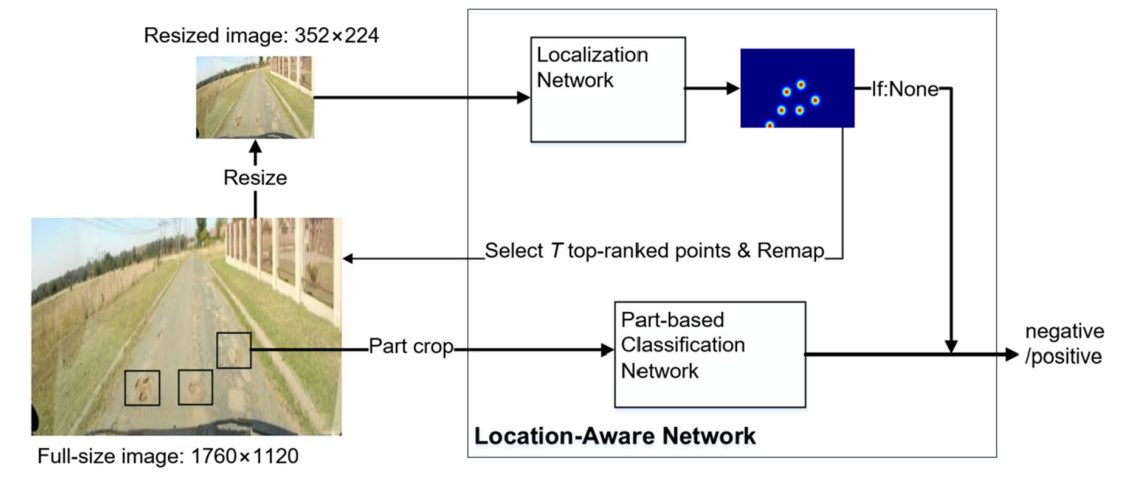
\includegraphics[scale=0.7]{Figures/chapter2/vision1.png}
    \caption{overview of location-aware network approach}
    \label{fig:my_label}
\end{figure}

\noindent
Traditional practices of median and Gaussian filtering,
connected components and binary image conversion had been
applied to recognize speed bumps, mostly to those road areas
where speed bump built with small height example of one such study is the Real Time Speed Bump Detection Using Gaussian Filtering and Connected Component Approach \cite{R13}. The proposed method uses Gaussian filtering and Median filtering to remove noise in the image. Subsequently, image subtraction is achieved by subtracting the Median filtered image from Gaussian filtered image. The resultant image is converted to a binary image and the regions are analyzed using connected component approach. The prior work on speed bump detection is achieved using sensors which are failed to detect speed bumps that are constructed with small height and the detection rate is affected due to erroneous identification. And the smartphone and accelerometer methodologies are not perfectly suitable for real-time scenarios due to GPS error, network overload, real-time delay, accuracy and battery running out. The proposed system goes very well for the roads which are constructed with proper painting irrespective of their dimension.

\noindent
In particular, this methodology suits very well the real time scenario for the painted speed bump though their pattern, color and dimensionality and road condition varies. In addition, it partially identifies illegal speed bumps (speed bumps that falls under category 5). This methodology is robust and effortless to implement in standalone machine that avoids congestion in networking (GPS), saving battery of smartphones while driving. The future scope of the proposed work is detection of bumps in night vision and bad illumination condition like raining and mist.

\noindent
The next paper proposes a method that detects and informs the driver about the upcoming un-marked and marked speed hump/bump in real time using deep learning techniques and gives the distance the vehicle is away from it using stereo-vision approaches. Here they have achieved this using NVIDIA GPU and Stereolab's ZED Stereo camera hardware\cite{R14}. With this driver or autonomous mode of the vehicle can control the vehicle speeds to be at safer limits in order to not cause any kind of discomfort to the passengers as well as damage to the vehicle  This is  achieved by the real-time early detection of marked and un-marked speed humps/bump using deep learning model and distance estimation using ZED stereo camera tested on laptop at 30 frames per second. here by deployed TensorFlow trained deep learning model on to android mobile as app and achieved real-time detection of bump at 2 frames per second. The robust testing of model was carried out on marked and unmarked speed breakers with partially faded paintings, covered by dust, shadows of trees and during night under street lightening conditions. The detection accuracy of proposed model is 97.44\% with false positive rate of 0.0427 for marked speed breakers, accuracy of 93.83\% with false positive rate of 0.0909 for un-marked speed breakers. The distance towards speed breaker is estimated with an accuracy of ±20cm in range of 2-10m. ZED camera doesn’t use IR, but uses color images for depth perception. So the detection of hump is poor at very lowlight environments. It was observed speed hump detection capabilities of the model were becoming low above 14m onwards as the object becomes smaller in the frame captured from the road scene. By use of models like faster RCNN which need little higher computational power but performs exceptionally well on smaller object detections, the distance estimation and can be improved till 20m with ZED camera.

\begin{figure}[h]
    \centering
    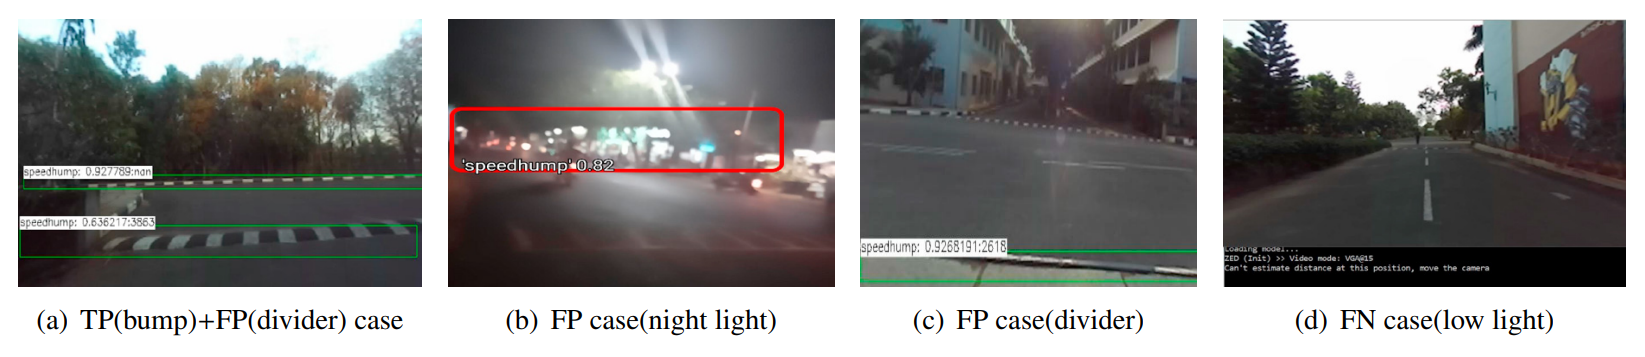
\includegraphics[scale=0.48]{Figures/chapter2/literature_results1.png}
    \caption{ Results of hump/bump detection and distance estimation}
    \label{fig:lit_res}
\end{figure}


\noindent
The next related study is Pothole and Bump detection using Convolution Neural Networks.In this paper an attempt to identify the road surface by classifying it into potholes, speed bump and normal roads based on image data\cite{R8}. The method of classifying the road surface from the images using convolution neural networks, ResNet-50 is discussed. Initially the images are manually classified into three classes and these are used to train the neural network, we were able to achieve a true positive rate of 88.9\%. In the second phase we pass the image to object detection neural network to detect the precise location of the speed bump. This was achieved using the YOLO algorithm for object detection. This work can be extended to alert the driver and tune the suspension to make the ride more comfortable based on road preview using a camera.Machine Learning based approaches can be used to detect pothole and speed bumps using images as opposed to sensor-based methods like accelerometers. This approach makes the method independent of the vehicle platform and can be easily implemented on any vehicle. Since the pothole and bumps are identified upfront, we can take preventive measures and make the ride safe and comfortable. It will be beneficial to consider more input images to cover a wide range of scenarios like rains, low light conditions, different road surfaces, etc. 

\noindent
The main limitation in this paper was that the
network can be made more robust by giving more input images,
training it for a longer time, and tuning the hyper-parameters. The number of input images used during the study did not cover a wide range of scenarios like rains ,low light conditions , different road surfaces etc.The next one was here was the data collection. To make the network more robust we need to gather more data and label the same which was not done.


\noindent
 In this paper,  an efficient pothole detection system is proposed using deep learning algorithms which can detect potholes on the road automatically\cite{R15}. Four models are trained and tested with preprocessed dataset, including YOLO V3, SSD, HOG with SVM and Faster R-CNN. In the phase one, initial images with potholes and non-potholes are collected and labeled. In the phase two, the four models are trained and tested for the accuracy and loss comparison with the processed image dataset. Finally, the accuracy and performance of all four models are analyzed. The experimental results show that the YOLO V3 model performs best for its faster and more reliable detection results. 

\begin{table}[h]
\begin{center}
  \begin{tabular}{|l|l|l|l|l|}
\hline
\textbf{Size} & \textbf{YOLOv3} & \textbf{SSD} & \textbf{HOG} & \textbf{Faster-RCNN} \\ \hline
200 images    & 53\%            & 47\%         & 24\%         & 72\%                 \\ \hline
650 images    & 67\%            & 59\%         & 25\%         & 71\%                 \\ \hline
850 images    & 65\%            & 55\%         & 27\%         & 67\%                 \\ \hline
1000 images   & 69\%            & 59\%         &              & 69\%                 \\ \hline
1100 images   & 73\%            &              &              & 60\%                 \\ \hline
1500 images   & 82\%            & 80\%         &              & 74\%                 \\ \hline
\end{tabular}  
\end{center}

\caption{Comparison of accuracy of different models}
\label{tab:my-table}
\end{table}

\noindent
Two of the limitations of the study were that they inferred YOLO V3 is the fastest but has the lowest accuracy which is not taken into consideration during the study while comparing the models and If the size of the potholes are large then the performance of the SSD is similar to that of YOLO V3.


\section{3D point cloud-based approaches}
Obtaining significant features of point cloud data consisted
the calculation of height variation, intensity of laser points,determining the z point (in 3D plane), road surface roughness representation and data point intensities in two diverse color spaces. These features were processed and examined the height of data points and the change of slope to the road boundaries\cite{R16}. 
\begin{figure}[H]
    \centering
    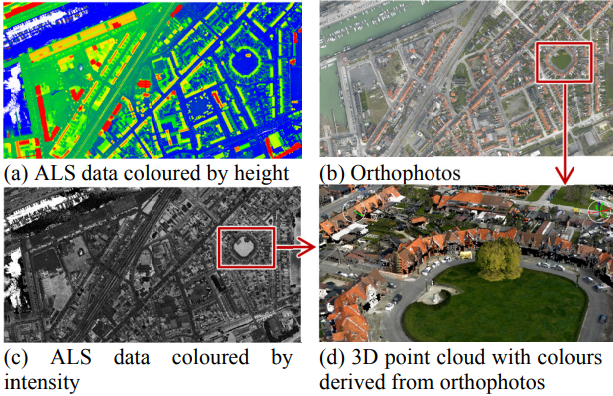
\includegraphics{Figures/chapter2/3dmethod1.png}
    \caption{ALS,Aerial Imagery data and the fusion Results}
    \label{fig:3d1}
\end{figure}

\noindent
This paper presents a workflow including a novel algorithm for road detection from dense LIDAR fused with high-resolution aerial imagery data. Using a supervised machine learning approach point clouds are firstly classified into one of three groups: building, ground, or unassigned. Ground points are further processed by a novel algorithm to extract a road network. The algorithm exploits the high variance of slope and height of the point data in the direction orthogonal to the road boundaries. Applying the proposed approach on a 40 million point dataset successfully extracted a complex road network with an F-measure of 76.9%. 

\noindent
J. Byun et al. applied markov random field (MRF) to differentiate between drivable and non-drivable road area. The computed feature vector formulation is then approximated to the goal region using principal component analysis (PCA) on the neighborhood covariance matrix \cite{R17}. In this paper, a novel method is proposed for road recognition using 3D point clouds based on a Markov random field (MRF) framework in unstructured and complex road environments. The proposed method is focused on finding a solution for an analysis of traversable regions in challenging environments without considering an assumption that has been applied in many past studies; that is, that the surface of a road is ideally flat. The main contributions of this research are as follows: (a) guidelines for the best selection of the gradient value, the average height, the normal vectors, and the intensity value and (b) how to mathematically transform a road recognition problem into a classification problem that is based on MRF modeling in spatial and visual contexts. In the proposed  experiments, they used numerous scans acquired by an HDL-64E sensor mounted on an experimental vehicle. The results show that the proposed method is more robust and reliable than a conventional approach based on a quantity evaluation with ground truth data for a variety of challenging environments. 
\begin{figure}[H]
    \centering
    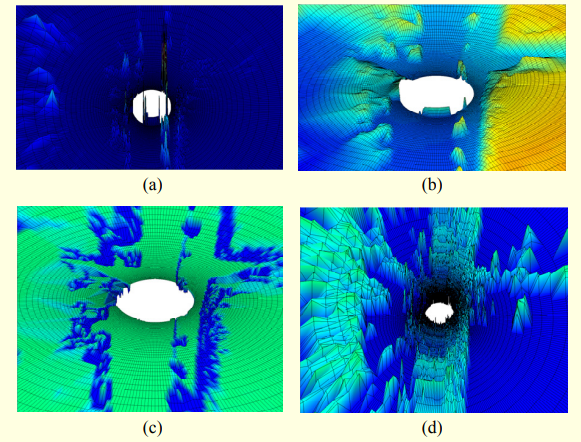
\includegraphics{Figures/chapter2/3dmethod2.png}
    \caption{Display of 3DGI features: (a) gradient value,(b)height value, (c) cosine similarity, and (d) intensity value.}
    \label{fig:3d2}
\end{figure}

\noindent
On the other hand, Suzzane et al. measured dimension of speed bump type of objects using the carrier frequency which was operated with interferometric approach on 24 GHz. This scheme assured a substantial level of sensitivity and appropriate for related types of application \cite{R19}.
This paper shows that an interferometric radar system operating at 24 GHz could be used for
automotive environment awareness in a context of unmanned ground vehicle applications.
The results show that the system can measure the height of small road objects, which tend to
be some number of centimeters high, with good precision using an interferometric technique
allied with SFCW modulation.
The experiments were performed at 24 GHz using two horn antennas for transmitting and
receiving, respectively. We used a vertical linear positioner in order to create many virtual
baselines in the processing, and a horizontal motor rail to measure the targets from different
range positions. Therefore, a model of an automotive scene was created in an indoor
environment. This technique could be used for autonomously driven car applications, as it could
detect small objects on the road and avoid vehicle damage or more serious accidents.




\noindent
As well as 
Surface modelling used the mobile laser scanning (MLS) to yield an even surface and thus the depth representation within reachable and feature-conserving framework got improved \cite{R20}This research work introduces the AGSR algorithm designed to supply scalable and detail-preserving ground surface reconstruction in a fully automatic fashion. 
\noindent
The
proposed technique generates accurate 3D models of outdoor environments adapted for the driving simulator
engine or for being embedded onboard mobile platforms
for autonomous navigation applications.
The reported technique addresses several open issues of
the currently existing surface reconstruction techniques,
such as accurate reconstruction of sharp depth features in
the presence of noisy datasets, scalability, and memory
usage.
Research perspectives of the present research work are
focusing on the photorealist surface reconstruction problem through the joint use of laser reflectance and RGB
cameras. A second research perspective is related to the
facade surface reconstruction and ground–facade merging
within a global referential frame






\section{DeepBus method(ML and IoT) }
This paper proposes a
machine learning based pothole detection system called DeepBus for real time identification of surface irregularities on roads using Internet of Things (IoT)\cite{R21}. DeepBus uses IoT sensors to detect potholes in real time while an end user is driving vehicles on the road. The location of these potholes would be available on a centrally hosted map which can be accessed by both end users and civic authorities. Thus, it would serve as a warning system to all users as well as a database of potholes with thier locations to the authorities for quick repair and action. They have compared the performance of various machine learning models (Logistic Regression, Support Vector Machine (SVM), K-Nearest Neighbors (KNN), Naive Bayes, Decision Tree, Random Forest and Ensemble Voting) based on different parameters (Accuracy, F-score, Precision and Recall) and identified that Random Forest is the best model for pothole detection.Here the live data of these potholes is made available through a real time map for all users to enable smart transportation. With this data, warnings can be given to drivers and their locations shared with civic authorities for quick repair. 





\noindent
Various future improvements can definitely be made to improve and expand the scope of DeepBus. If the system can
differentiate and classify speed bumps it would further add functionality to the DeepBus. Apart from marking potholes,
developing a system to map road conditions would help drivers make more informed choices. Next feature can be added to classify the severity of a pothole. Differentiating a deep pothole with a shallow one will enable Governments to assign priorities while fixing potholes. Another important future direction is reducing misclassifications. A misclassified pothole is detrimental and a waste of time and money to authorities as well as users.

\noindent
 Drawbacks of DeepBus was that the system cannot differentiate and classify speed bumps using the DeepBus method which can be very beneficial.Sensor based approaches may not portray the actual scene effectively, producing a malformed pattern at specific points which are comparatively higher than the actual estimation thus may lead to false detection in given scenario.
